\documentclass[oneside]{book}

\usepackage{fullpage,hyperref,titlesec,enumerate,babelbib,graphicx,float}
\usepackage[english]{babel}
\usepackage{titlesec} % required for removing header spacing

% remove header spacing
\titlespacing\section{0pt}{12pt plus 4pt minus 2pt}{0pt plus 2pt minus 2pt}
\titlespacing\subsection{0pt}{12pt plus 4pt minus 2pt}{0pt plus 2pt minus 2pt}
\titlespacing\subsubsection{0pt}{12pt plus 4pt minus 2pt}{0pt plus 2pt minus 2pt}

% remove all indents
\setlength{\parindent}{0pt}

% Add all chapter folders to graphics path
\graphicspath{
 {./profiling/}
}

\titleformat{\chapter}[hang]{\Huge\bfseries}{\thechapter. }{0pt}{\Huge\bfseries}

\begin{document}
\frontmatter
%%% TITELPAGE %%%

\begin{titlepage}

\begin{center}
\begin{figure}[h!]
\centering
% Title image
% \includegraphics[scale=1]{Images/TU_P2_black.png}
\end{figure}
Faculty of Computer Science \\
\today

\vspace{3.5cm}
\selectfont
{\Large TN3706 - Bachelor Seminar}\\
\vspace{0.0cm}
\Huge{\textbf{Performance Regression Testing\\ A developer's perspective}}
\vspace{0.5cm}
\selectfont

\vspace{5cm}
\normalsize{\textbf{Bachelor Seminar Group}}

\begin{tabular}{ l r}
\normalsize{M.A. Hoppenbrouwer} & \normalsize{4243889} \\
\normalsize{M.J. Otte} & \normalsize{4222695} \\
\normalsize{R.S. Sluis} & \normalsize{4088816} \\
\normalsize{R. Vink} & \normalsize{4233867}\\
\end{tabular}

\vspace{0.75cm}

\begin{tabular}{ l l }
\normalsize{M. Loog} & \normalsize{Professor} \\
\normalsize{C. Bezemer} & \normalsize{Supervisor} \\
\end{tabular}

\end{center}
\end{titlepage}

\chapter{Preface}
% In the growing world of tools and methods that are available to a software developer, it becomes harder and harder to keep track of which technique is best to use under what circumstances. This holds true for the growing field of performance regression testing, where new testing strategies are being discovered and discussed, and the steps in the process of detecting performance regressions are being improved constantly. This literature study aims to give an overview of these steps in a way that links each step to a point in the software development process corresponding to the challenges that arise when dealing with performance regression testing in practice.


\chapter{Summary}
% Performance regression testing brings challenges with it. In this paper we discuss what these challenges are, how they are handled and what problems still remain. It shows when it is useful to start performance regression testing during the development. How the data for the tests are gathered. What can be done to process the gathered data. And how to report on it. Ultimately there is still work to be done in the subject, but the paper shows that performance regression testing is a useful method of testing.


\clearpage % To point the bookmark to the top of the page
\pdfbookmark{\contentsname}{toc}
\tableofcontents

\clearpage % To point the bookmark to the top of the page
\pdfbookmark{\listfigurename}{lof}
\listoffigures

\clearpage % To point the bookmark to the top of the page
\pdfbookmark{\listtablename}{lot}
\listoftables

\mainmatter
%  INTRODUCTION
% The definition of performance regression testing is: ``Performance regression testing detects performance
regressions in a system under load. Such regressions refer to
situations where software performance degrades compared to
previous releases, although the new version behaves correctly.''\cite{foo2010mining}
Performance regression testing can be seen as the combination of regression testing and performance testing. ``Regression tesing is the retesting of software following modifications.''\cite{rothermel2001prioritizing} Performance testing is testing performance requirements and specifications of it.\cite{gan2006software}

To improve the quality of the software product it could be useful to use performance regression testing in a way the developers can
directly improve the quality of the software product. This will be the main focus of this article. There are different aspects in optimizing performance regression tests, which will be discussed throughout this paper. Every aspect will be clarified in the form of a new chapter in this paper. \\ First of all it needs to be clear how to acquire data and what kind of performance counters will be used for performance regression testing. Next is the filtering of the performance metrics, used to obtain differences in data. The following chapter discusses how to compare the filtered data. Last aspect is that the filtered performance metrics can be reported in the form of visualizations so performance regressions will be detected. At the end of this paper, a research agenda and a conclusion will be provided.



\chapter{Definition of PRT}
\label{chapter:definition}
The following chapter will explain the definition of performance regression testing (PRT). PRT is the combination of regression testing with performance testing. First we will explain what regression testing is, then what performance testing is and last we will discuss what the combination of the two means.

\section{Definition of regression testing}
Regression testing tests whether or not the software has new regressions, software bugs, each time a software change or update is made. Regression testing also determines if software changes made in one part of the software affects the other parts. Usually software bugs will occur when the software is updated. That is why regression testing is used a lot nowadays. Regression testing is applied by running the old test scenarios for the changed program. These tests will cover all the functions and input so that every situation will be tested.

\section{Definition of performance testing}
Performance testing is testing in a way so that performance quality won't be lost. Programmers make certain performance demands and test whether or not these demands are fulfilled. For example the time the program takes to log in must be shorter than 1 second. If the software is not able to achieve this demand, the software has to be adjusted.

\section{Definition of PRT}
The combination of performance testing and regression testing is PRT. This means that if software is tested, it will make sure that regressions will be detected and the loss in performance will be registered.

Regression testing focuses on the verifying of correctness of a change \cite{detection_performance_regressions}. Some large researches actually show that performance is most of the time the biggest primary problem in the field \cite{Mining_PRT_Automated}. \newline To improve the quality of the software product it could be useful to use PRT in a way the developers can directly improve the quality of the software product. A timeline when to make use of PRT in the development process could be useful.


\chapter{Time of Performing PRT}
\label{chapter:timeline}
To show when in the developing process we will try to apply PRT, we will make a timeline. The timeline contains all the phases of a software development process. The software development processes are different for each kind of approach. For this research we will make a timeline using the SCRUM development process.
\section{Scrum}
\subsection{Definition of Scrum}
SCRUM is a development process named to the rugby method of play. In rugby it means that a formation will group together to gain the ball as fast as possible. For the developing this means that a group of people work in short sprints to realize the desired software product as soon and as safe as posible.
\subsection{Phases of Scrum}
SCRUM contains 3 kind of phases. The planning and closure phases consist of knowing the input and output of the project. These phases are just organising phases, so not much developing will be made. The development will take place during the sprints which can be divided in developing, wrapping, reviewing and adjusting. This is a continuous process which will finish once the project is in the closure phase. Developing is where the programming will be done, then wrapping is done to combine all the elements of the development process, reviewing is done to make sure if the process is working well and adjusting is the phase to improve the implemented functions. Sprints are in cycles, so after the adjusting phase, the developing phase will be the next phase, so that the cycle is complete.

\begin{figure}[h]
\begin{center}
	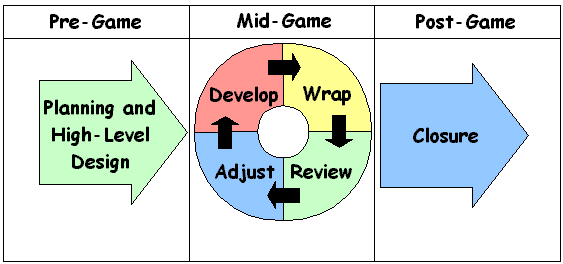
\includegraphics[width=0.5\textwidth]{Figures/diagram01.png}
\end{center}
	\caption{phases of scrum}

\end{figure}

\section{Time of PRT using SCRUM} Now we can choose where in the development process PRT will take place. The planning and closure phases are not suitable for PRT, because these phases are just organising phases. The other phase consists of the sprints. During the sprints all the developing tasks will be done, so this will be the right phase to performance regression test. Research has been done to show that automated regression tests during the daily builds will greatly improve the quality of the product \cite{Future_of_Scrum}. Regression testing was done during the wrapping phase of the sprints of Scrum. In the end they made sure that everything was tested for regressions yet again, to make sure the product was ready to ship.

\section{Appointing one person to test performance regressions} Another research team appointed one person of the developing group to continuously watch over the quality of the software product \cite{Fully_Distributed_Scrum}. This person is an active member of the team and watches all the members of the developing team. This method provides a way to deal with any issues that could come up during the process. The appointed person will directly try to deal with issues coming up by the members of the developing team. By appointing this person, the quality of the product is watched the whole time during the project, instead of comparison to the other research where PRT is done during the merge phase. This research proved that the quality of the development got a much higher average score compared to other similar development products. So appointing one tester who only has the task to watch over the quality by testing and for our sake performing regression tests, has an improved effect on the overall process.

\section{}



\chapter{Performance Counters}
\label{chapter:performancecounters}
\section{Performance counters}

This chapter discusses how perfomance counters can give information about the quality of software. Performance counters are a type of data output as a result of performance regression testing. Performance counters can count different types of events like CPU utilization, memory utilization or disk IO.

\subsection{Results of performance counters}
To detect if performance regression occurs, the results of the prior and the new performance regression test need to be compared. "A performance regression means that the new version uses more resources or has less throughput than prior versions" \cite{DetectionPerformanceRegression}. The results of these tests can be analyzed manually, but this costs a lot of time. A faster approach would be to use a control chart. A control chart consists of a baseline data set and a target data set. A baseline data set contains the results of the prior test. Based on this data set an upper and lower limit will be decided. The target data set contains the results of the new test. From these two data sets the violation ratio can be calculated. This is the percentage of the amount of targets outside the upper and lower limit. If performance regression occurs, the violation ratio is too high. It now seems easy to detect if performance regression occurs: a certain threshold on the maximum allowed violation ratio can be chosen, and if the violation ratio is higher than this threshold performance regression has occurred. Unfortunately, this is not the case. There are some things that make it hard to detect performance regression. If the violation ratio is low, the probability that performance regression has occurred is low as well. A high violation ratio doesn't always mean that performance regression has occurred. Some performance counters are inconsistent, and show different results on the same input data. Because of this, it is possible that the violation ratio is higher than the chosen threshold but no performance regression has occurred. To avoid this, the prior test will be executed again after the new test.

\subsection{Accuracy of performance counters}
But how accurate are the results of performance counters? What techniques can make these results more accurate?

Experiments have shown that "reducing the number of concurrently measured hardware events can be a good way to improve measurement accuracy"\cite{AccuracyPerformanceCounter}. However, this depends on some factors, for instance the type of interface that is used, or the counter configuration.
Tests with different interfaces (perfmon2 and perfctr) and different counter configurations (user and user+kernel) show that for the combination of the perfmon2 interface and user+kernel configuration the measurement error increases as the number of registers increases as well. \cite{AccuracyPerformanceCounter}
Also, the type of infrastructure is very dependent. The measurement error reduces a lot when a low-level infrastructure is used, instead of a high-level infrastructure.
On top of that, for the user+kernel mode the measurement error gets bigger if the duration of the benchmark gets longer. \cite{AccuracyPerformanceCounter} So to make the measurement error smaller, less loop iterations should be used.  The infrastructure doesn't have influence. For the user mode the duration of the benchmark doesn't matter. This is because of interrupts, that only occur in kernel event counts. More interrupt-related instructions will include if the duration of a measurement takes longer.



\chapter{Profiling}
\label{chapter:profiling}
The following section describes the role of profiling in performance regression testing. The first section explains what profiling is and how it can be applied to draw meaningful conclusions about large volume of results produced by performance regression testing.

\section{The role of profiling}
Profiling plays an important part in performance regression testing. As described in Chapter [link here], a lot of data is produced when a software application is submitted to performance tests. Chapter [link here] discusses the use of performance counters to separate the significant parts of that data from the bulk of it. The next step is making sense of this data, which is where profiling comes in. To understand what profiling is and how it is used, a few perspectives on performance profiling are provided first.

\subsection{Different uses of profiling}
Bezemer et al. look into creating a comparable profile of the performance of a piece of software \cite{io_regressions}. In particular they focus on guiding performance optimization when there are factors in play such as multiple software languages and varying test performance due to system resources being (un)available during some tests, but not others.

Ghaith et al. use profiling as a way to model the performance of a system, particularly distributed systems, by using Transaction Profiles as a load-independent representation of transaction response time \cite{profile_based_detection}. The method relies on the representation of the system as a queueing network, which can be used to model a number of different systems of high complexity \cite{performance_puzzles}.

The common factor in the different uses of profiling discussed above is the following: a performance profile can be used to track performance changes over different releases, detect performance regressions and identify the responsible factors in the corresponding software. The prerequisite to this is that the profile has to be comparable, and thus representative of its software counterpart, which for the remainder of this chapter will be assumed to be the case since a non-comparable profile would serve no purpose in performance regression testing.

\subsection{Profiling in relation to performance regression testing}


\section{Profiling techniques and factors}



% CONCLUSION
\newpage
% This paper shows that performance regression testing could help the developer improve their system. To do so the developer needs to gather performance metrics, process this data and draw meaningful conclusions from it. If all these steps are made, the developer can tell what kind of performance regressions have occurred, so they can adjust their system. Performance regression testing is a rather new subject in the field Computer Science. This means that it can be further investigated. Some of these future experiments can be found in the research agenda.


% Appendices
\appendix


% END appendices

\backmatter

\phantomsection
\addcontentsline{toc}{chapter}{\bibname}

\bibliographystyle{unsrt}
\bibliography{bibliography}

\end{document}
